% Preamble
\documentclass[12pt, a4paper]{article}
\usepackage[bahasa]{babel} % For Bahasa Indonesia
\usepackage{times} % For Times New Roman
\usepackage[utf8]{inputenc} % Input encoding
\usepackage[T1]{fontenc} % Font encoding
\usepackage{amsmath} % For math
\usepackage{amssymb} % For math symbols
\usepackage{graphicx} % For images
\usepackage{caption} % For captions
\usepackage[left=3cm, right=3cm, top=3cm, bottom=3cm]{geometry} % Margins
\usepackage{setspace} % For line spacing (1.5 spacing)
\usepackage{titlesec} % For customizing section titles
\usepackage{textcomp} % For text symbols like \textsuperscript
\usepackage{xurl} % For handling URLs in references, allows breaks
\usepackage{ragged2e} % For \justify command
\usepackage{enumitem} % For customizing lists

% Custom command for Abstract/Abstrak titles (11pt bold, all caps)
\newcommand{\makecustomsectiontitle}[1]{{\centering\normalfont\fontsize{11}{13}\selectfont\bfseries\MakeUppercase{#1}\par}\vspace{1em}\nopagebreak}

% Global line spacing (uwe.md: "1.5 spaced (Eng)")
\onehalfspacing % uwe.md: "1.5 spaced (Eng)"

% Section title formatting (uwe.md: "12 bold, capital")
% Unnumbered sections, as per general academic article style for these top-level headings
\titleformat{\section}
  {\normalfont\fontsize{12}{14}\bfseries\MakeUppercase}
  {} % no number
  {0em} % no separation
  {}[
\vspace{0.5ex}] % code before, space after title
\titlespacing*{\section}{0pt}{*3}{*2} % left, before, after spacing. *3 means 3 lines of space before

% Subsection title formatting (uwe.md: "Subchapter...Capital letter for the initial word")
% Unnumbered, 12pt bold.
\titleformat{\subsection}
  {\normalfont\fontsize{12}{14}\bfseries}
  {} % no number
  {0em} % no separation
  {}[
\vspace{0.5ex}]
\titlespacing*{\subsection}{0pt}{*2}{*1.5}

% Sub-subsection title formatting (uwe.md: "Sub-subchapter...Capital letter for the initial letter and italic")
% Unnumbered, 12pt bold italic.
\titleformat{\subsubsection}
  {\normalfont\fontsize{12}{14}\bfseries\itshape}
  {} % no number
  {0em} % no separation
  {}[
\vspace{0.5ex}]
\titlespacing*{\subsubsection}{0pt}{*2}{*1.5}

% Justification for main text
\Justifying

\begin{document}

% Title Page elements
\begin{titlepage}
    \centering
    \vspace*{\stretch{1}} % Pushes content down
    {\fontsize{16}{19}\bfseries\selectfont Bagaimana dinamika historis dan urgensi wawasan nusantara sebagai konsepsi dan pandangan kolektif kebangsaan indonesia dalam konteks pergaulan dunia\par} % Title from main.typ, Times New Roman 16pt
    \vspace{1cm} % Space after title
    {\fontsize{11}{13}\bfseries\selectfont Nama Penulis Pertama$^1$, Nama Penulis Berikutnya$^2$, Nama Penulis Terakhir$^3$\par} % Placeholder authors, Times New Roman 11pt bold
    \vspace{0.5cm} % Space after authors
    {\fontsize{10}{12}\selectfont $^1$Institusi Penulis Pertama\par} % Placeholder institutions, Times New Roman 10pt
    {\fontsize{10}{12}\selectfont $^2$Institusi Penulis Berikutnya\par}
    {\fontsize{10}{12}\selectfont $^3$Institusi Penulis Terakhir\par}
    \vspace{0.3cm}
    {\fontsize{10}{12}\selectfont Corresponding author: email@example.com\par} % Placeholder email
    \vspace*{\stretch{2}} % Pushes content up from bottom
\end{titlepage}
\clearpage
\pagenumbering{arabic} % Start page numbering for the main content

% ABSTRACT (English)
\makecustomsectiontitle{ABSTRACT}
\singlespacing % uwe.md: 1 space for abstract, Times New Roman 10pt, Italic, and Justify
\begin{justify}
\fontsize{10}{12}\selectfont\itshape
Abstract should be factual and concise. It should be written in English and Bahasa. It shall contain research problems, purpose, methods, and results. Please do not change the format (Times New Roman 10pt, Italic, and Justify). Maximum length 150 - 250 words.
\par\vspace{0.5em}
\textit{Keywords:} keyword1, keyword2, keyword3, keyword4, keyword5 % use 10 pt, times new roman, Italic
\end{justify}
\onehalfspacing % Return to default spacing
\vspace{1cm}

% ABSTRAK (Bahasa Indonesia)
\makecustomsectiontitle{ABSTRAK}
\singlespacing % uwe.md: 1 spasi, Times New Roman 10pt, dan Justify. Example image also has italic.
\begin{justify}
\fontsize{10}{12}\selectfont\itshape % uwe.md example image shows italic
Wawasan nusantara merupakan cara pandang bangsa terhadap diri dan lingkungan tempat hidup bangsa yang bersangkutan. Cara bangsa memandang diri dan lingungannya sangat mempengaruhi keberlangsungan dan keberhasilan bangsa itu menuju tujuannya. Berdasarkan lembaga ketahanan nasional tahun 1999 pengertian wawasan nusantara adalah sebuah cara pandang dan sikap bangsa indonesia mengenai diri dan lingkungannya yang serba beragam dan bernilai strategis dengan mengutamakan persatuan dan kesatuan bangsa serta kesatuan wilayah dalam penyelenggaraan kehidupan bermasyarakat, berbangsa dan bernegara untuk mencapai tujuan nasional.
\par\vspace{0.5em}
\textit{Kata Kunci:} wawasan nusantara, geopolitik, indonesia, persatuan, kesatuan % penggunaan 10 pt, Times New Roman, diurutkan sesuai abjad
\end{justify}
\onehalfspacing % Return to default spacing
\vspace{1cm}

% INTRODUCTION - PENDAHULUAN (uwe.md: "without subsection", "Times New Roman 12pt, 1.5 spaced (Eng)")
\section*{INTRODUCTION - PENDAHULUAN}
\setlength{\parindent}{1em} % Standard paragraph indent for the main text sections
Wawasan nusantara ini bisa dibagi menjadi dua pengertian yakni pengertian secara etimologis dan pengertian terminologi.

\textbf{1. Etimologi}

Secara etimologi, kata wawasan nusantara berasal dari dua kata wawasan dan nusantara. wawasan dari kata wawas (Bahasa jawa) yang artinya pandangan. sementara kata "nusantara" merupakan gabungan kata nusa yang artinya pulau dan antara. kata "nusa" dalam bahasa sansekerta berarti pulau atau kepulauan. dan kata "Antara" memiliki padanan dalam bahasa latin, \textit{in } dan \textit{terra} yang berarti antara atau dalam suatu kelompok, kata nusantara dapat diartikan sebagai kepulauan yang diantara laut atau bangsa-bangsa yang dihubungkan oleh laut. Kata nusantara sendiri bermula dari bunyi Sumpah Pala dari Patih Gajah Mada yang diucapkan dalam upacara pengangkatannya sebagai Mahapatih di Kerajaan Majapahit tahun 1336 M, Tertulis di dalam Kitab Paraton. bunyi sumpah tersebut sebagai berikut:
\begin{quote}
\itshape Gajah Mada Patih Amangkubumi tidak ingin melepaskan puasa. Ia Gajah Mada, “Jika telah mengalahkan nusantara, saya (baru akan) melepaskan puasa. Jika mengalahkan Gurun, Seran, Tanjung Pura, Haru, Pahang, Dompo, Bali, Sunda, Palembang, Tumasik, demikianlah saya (baru akan) melepaskan puasa”.
\end{quote}
Penamaan Nusantara ini berdasarkan sudut pandang Majapahit (Jawa), mengingat pada waktu itu belum ada sebutan yang cocok untuk menyebut seluruh kepulauan yang sekarang bernama indonesia dan juga Malaysia. Kemudian Kata Nusantara digunakan oleh Ki Hajar Dewantara untuk menggantikan sebutan Hindia Belanda (\textit{Nederlandsch-Indie}), pada acara Kongres Pemuda Indonesia II tahun 1928 (peristiwa Sumpah Pemuda), digunakan istilah Indonesia sebagai pengganti Nusantara. Nama Indonesia berasal dari dua kata bahasa Yunani, yaitu \textit{indo/indu} yang berarti Hindu/Hindia dan \textit{nesia/nesos} yang berarti pulau. Dengan demikian kata nusantara bisa dipakai sebagai sinonim kata indonesia, yang menunjuk pada wilahay (sebaran pulau-pulau) yang berada di antara dua samudra yakni Samudra Hindia dan Samudra Pasifik dan dua benua yakni Benua Asia dan Australia.

\textbf{2. Terminologis}

Untuk Pengertian terminologis, wawasan nusantara merupakan pandangan bangsa indonesia terhadap lingkungan tempat berada termasuk diri bangsa Indonesia itu sendiri. Rumusan Wawasan Nusantara dalam GBHN 1998:
\begin{quote}
\itshape “Wawasan Nusantara adalah cara pandang dan sikap bangsa Indonesia mengenai diri dan lingkungannya, dengan mengutamakan persatuan dan kesatuan bangsa serta kesatuan wilayah dalam penyelenggaraan kehidupan bermasyarakat, berbangsa dan bernegara”.
\end{quote}

\textbf{Latar Belakang Historis Wawasan Nusantara}

Lahirnya Konsepsi wawasan nusantara bermula dari Perdana Menteri Ir. H. Djuanda Kartawidjaja yang pada tanggal 13 Desember 1957 mengeluarkan deklarasi yang selanjutnya dikenal sebagai Deklarasi Djuanda. isinya sebagai berikut:
\begin{quote}
\itshape "Bahwa segala perairan di sekitar, di antara dan yang menghubungkan pulau-pulau yang termasuk Negara Indonesia dengan tidak memandang luas atau lebarnya adalah bagian-bagian yang wajar daripada wilayah daratan Negara Indonesia dan dengan demikian bagian daripada perairan pedalaman atau nasional yang berada di bawah kedaulatan mutlak Negara Indonesia. Lalu lintas yang damai di perairan pedalaman ini bagi kapal-kapal asing dijamin selama dan sekedar tidak bertentangan dengan/mengganggu kedaulatan dan keselamatan Negara Indonesia. Penentuan batas landas lautan teritorial (yang lebarnya 12 mil) diukur dari garis yang menghubungkan titik-titik ujung yang terluar pada pulau-pulau Negara Indonesia. Ketentuan-ketentuan tersebut di atas akan diatur selekas-lekasnya dengan Undang-Undang"
\end{quote}
_yang intinya mendeklarasikan bahwa perairan di sekitar, di antara, dan yang menghubungkan pulau-pulau Indonesia adalah bagian dari wilayah daratan Indonesia. Ini mengubah pandangan sebelumnya yang berdasarkan Ordonansi 1939, di mana laut hanya diakui sejauh 3 mil dari garis pantai._ % This line was italic in source, kept it as such

Kemudian pada tanggal 30 April 1982, PBB mengeluarkan dokumen yang bernama \textit{"The United Nation Convention on the Law of the Sea"} (UNCLOS). yang mengakui indonesia sebagai negara kelautan yang memiliki wilayah laut sebesar 5.9 Juta km\textsuperscript{2}.

% Figure placement - User needs to ensure 'images/unclos.png' is accessible.
% The path in main.typ was: image("images/unclos.png")
% I'm commenting out includegraphics to prevent compilation errors if the image is missing or path is wrong.
% User should place final_exam.tex such that 'images/unclos.png' is found, e.g. in a subdirectory.
% \begin{figure}[htbp]
%     \centering
%     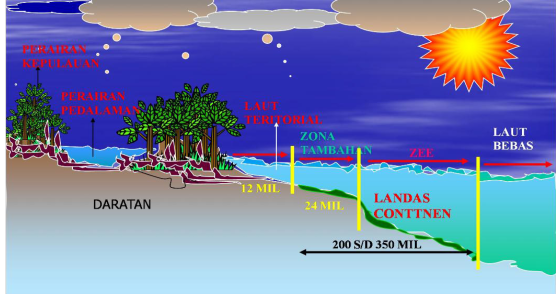
\includegraphics[width=0.8\textwidth]{images/unclos.png} % Ensure 'images' folder is in same dir as .tex or provide full/relative path
%     \caption{Gambar 1: grafik zona peraian indonesia berdasarkan konvensi hukum laut pbb 1992} % uwe.md: caption lowercase
%     \label{fig:unclos}
% \end{figure}
% User note: Please uncomment the figure environment above and ensure the image 'images/unclos.png' is correctly placed for compilation.

\textbf{Latar Belakang Sosiologis Wawasan Nusantara}

Pada awalnya Bangsa indonesia adalah bangsa yang terpecah belah dan berfokus pada masing masing suku dikarenakan di adu domba dalam masa penjajahan oleh Belanda yang disebut teknik politik \textit{Devide et Impera} yang mana kondisi sosial budaya indonesia hanya berputar pada satu golongan saja dan tidak ada kesatuan, namun kemudian mulainya keluar bibit bibit persatuan yang dimulai dengan peristiwa Kebangkitan Nasional pada Tanggal 20 Mei 1908 yang kemudian Ditegaskan kembali dalam Sumpah Pemuda pada 28 Oktober 1928 yang kemudian berhasil diwujudkan dengan proklamasi Kemerdekaan bangsa pada tanggal 17 Agustus 1945 yang berhasil menyatukan Indonesia, oleh karena itu sebelum Deklarasi Djuanda 1957 pun konsep semangat dan kesatuan kebangsaan sudah tumbuh dalam diri bangsa.

\textbf{Latar Belakang Politis Wawasan Nusantara}

Wawasan Nusantara menjadi konsep politik kenegaraan untuk mempertahankan kesatuan wilayah dan bangsa. Letak geografis Indonesia yang strategis, yaitu di antara dua benua (Asia dan Australia) dan dua samudra (Hindia dan Pasifik), juga memengaruhi pandangan geopolitik Indonesia.

% METHODS - METODE PENELITIAN (uwe.md: "There is no methodology for non research papers")
\section*{METHODS - METODE PENELITIAN}
Bagian ini menjelaskan metodologi penelitian yang digunakan (jika ada). Sesuai panduan, untuk artikel non-penelitian, bagian ini dapat disesuaikan atau dihilangkan jika tidak relevan.

% FINDINGS AND DISCUSSION - HASIL DAN PEMBAHASAN (uwe.md: Subchapters allowed)
\section*{FINDINGS AND DISCUSSION - HASIL DAN PEMBAHASAN}

\subsection*{Esensi dan Urgensi Wawasan Nusantara}
\subsubsection*{Esensi}
\begin{itemize}
    \item Kesatuan Wilayah: Indonesia sebagai negara kepulauan dengan 17.508 pulau.
    \item Persatuan bangsa: Keragaman suku, agama dan budaya harus dipandang sebagaii satu kesatuan.
\end{itemize}

\subsubsection*{Urgensi}
\begin{itemize}
    \item Mempertahankan keutuhan wilayah dan kedaulatan negara.
    \item Mencegah disintegrasi bangsa.
    \item Meningkatkan kesejahteraan rakyat melalui pengelolaan sumber daya alam yang adil dan merata.
\end{itemize}

\subsection*{Tantangan dan Potensi}
\subsubsection*{Potensi Positif}
\begin{itemize}
    \item Kekayaan sumber daya alam yang melimpah.
    \item Keragaman Ras, agama dan suku.
    \item Letak geografis strategis untuk perdagangan dan pertahanan.
\end{itemize}

\subsubsection*{Potensi Negatif}
\begin{itemize}
    \item Ancaman Disintegrasi akibat perbedaan suku, agama dan budaya.
    \item Masalah pembangunan yang tidak merata, dikarenakan karena geografi dan birokrasi, terutama di daerah tertinggal.
\end{itemize}

\subsection*{Implementasi Wawasan Nusantara}
% The source main.typ has these as simple list items. uwe.md sub-subchapter is italic. But these are more like bullet points under a subchapter.
% Let's keep them as a list for clarity.
\begin{itemize}
    \item \textbf{Politik:} Kesatuan wilayah dan bangsa dalam penyelenggaraan negara berdasarkan Pancasila dan UUD 1945.
    \item \textbf{Ekonomi:} Pembangunan ekonomi yang merata dan berkeadilan.
    \item \textbf{Sosial Budaya:} Menghargai keragaman budaya sebagai kekuatan bangsa.
    \item \textbf{Pertahanan dan Keamanan:} Ancaman terhadap satu daerah adalah ancaman terhadap seluruh bangsa.
\end{itemize}

% CONCLUSION - KESIMPULAN
\section*{CONCLUSION - KESIMPULAN}
Bagian ini merangkum temuan utama dan diskusi. Hindari pengulangan dari abstrak atau bagian sebelumnya. Kesimpulan harus menjawab tujuan atau hipotesis penelitian jika ada, serta memberikan implikasi atau rekomendasi berdasarkan hasil pembahasan.

% REFERENCES - DAFTAR PUSTAKA (uwe.md: APA style)
\section*{REFERENCES - DAFTAR PUSTAKA}
\begin{thebibliography}{99} % Increased number for more refs
\bibitem{affan2021} Affan, F. (2021). “Lazismu Distribusikan Daging Kaleng Qurban dalam Olahan Rendang”. Dalam \textit{Tribun Jateng}. Diakses pada 3 Oktober 2021 dari laman \url{https://jateng.tribunnews.com/2021/06/24/lazismu-distribusikan-daging-kaleng-qurban-dalam-olahan-rendang-target-himpun-dana-rp-42-miliar}
\bibitem{alwi2015} Alwi, M. M. (2015). Optimalisasi Fungsi Masjid dalam Pemberdayaan Ekonomi Masyarakat. \textit{Jurnal Al-Tatwir, 2}(1), 133-150.
\bibitem{chambers2006} Chambers, E., \& Gregory, M. (2006). \textit{Teaching and Learning English Literature}. London: Sage Ltd.
\bibitem{hanbal2001} Hanbal, A. A. B. M. B. (2001). \textit{Musnad Imam Ahmad Bin Hanbal}. Beirut: Ar-Risalah.
\bibitem{rozalinda2016} Rozalinda. (2016). \textit{Manajemen Wakaf Produktif}. Depok: PT. Raja Grafindo.
\bibitem{syamsudin2022} Syamsudin. (2022). “Pembagian Hasil Kurban Lazismu”. Hasil Wawancara Pribadi. Dilakukan secara daring melalui zoom meeting pada 16 Agustus 2022.
\bibitem{syihabuddin2011} Syihabuddin, A. (2011). \textit{Distribusi Kekayaan Studi Komparatif Pemikiran Baqir al-Sadr dan Taqiy al-Din al-Nabhan}. Tesis. Program Pascasarjana. Universitas Islam Negeri Sunan Ampel.
\bibitem{ulihanli2017} Uluhanli, L., et al. (2017). \textit{Masjid: Kemegahan Islam}. United States: Rizzoli Press.
% Add your actual references here following APA style
\end{thebibliography}

\end{document}
